\documentclass[10pt]{article}
\usepackage[utf8]{inputenc}
\usepackage{url}
\usepackage{hyperref}
\usepackage{amsmath}
\usepackage{amsfonts}
\usepackage{amssymb}
\usepackage{graphicx}
\graphicspath{ {./images/} }
\usepackage{float}
\usepackage{lipsum}
\usepackage{sectsty}
\sectionfont{\centering}
\usepackage{multicol}
\usepackage{xcolor}
\usepackage{natbib}
\usepackage{graphicx}
\usepackage{listings}
\usepackage{xcolor}
\usepackage[font=small]{caption}
\addtolength{\abovecaptionskip}{-3mm}
\addtolength{\textfloatsep}{-5mm}
\setlength\columnsep{20pt}

\usepackage[a4paper,left=1.50cm, right=1.50cm, top=2cm, bottom=3cm]{geometry}


\author{}

\title{\Large{Design and Analysis of Algorithms Assignment - 2}}
\begin{document}
	\begin{center}
		{\Large \textbf{Design and Analysis of Algorithms Assignment - 2}}\\
		\vspace{1em}
		{\large Department of Information Technology}\\
		\vspace{1em}
		\large{Indian Institute of Information Technology - Allahabad, India}\\
		\vspace{1em}
		\large{ Ritu Kiran Murmu(IIB2019025)      Atithi kumari(IIB2019026)     Shahid(IIB2019027)}
		\vspace{2.5em}
		
	\end{center}
	
\begin{multicols*}{2}

    \textbf{\emph{{Abstract}: In this paper ,we have designed an algorithm to find  the area of n- sided polygon. We have used the divide and conquer approach to solve the problem and also analysed the time and space complexity of the program.
}}\\
	
	\textbf{\emph{{Index Terms}: Arrays, Divide and Conquer\\}}


\section*{INTRODUCTION}
 
We have been given set of ordered points in 2D plane.An Array is a linear data structure which stores similar elements in contiguous memory locations. A Shoelace formula has been used on the array.

\paragraph{Divide and Conquer}
In divide-and-conquer  we try to decompose a given problem into two or more similar, but simpler, sub-problems, to solve them in turn, and to compose their solutions to find optimal solution of the problem. So, basic idea here is: 
\begin{enumerate}
    \item\textbf{Divide:} This involves dividing the problem into some sub problem.
    \item\textbf{Conquer:} Sub problem by calling recursively until sub problem solved.
    \item\textbf{Combine:} The Sub problem Solved so that we will get find problem solution.Let us have a pictorial look of the image which makes the concept of Divide and Conquer Paradigm self explanatory.\\\\
\end{enumerate}

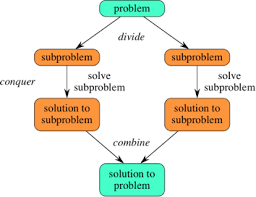
\includegraphics[width=\columnwidth, height=8cm]{dac.png}\begin{center}\textbf{Figure 1:} Divide and Conquer\end{center}


\paragraph{Advantages of Divide and Conquer}
The Divide and Conquer technique generally has following mentioned advantages over Brute Force Algorithms.\\\\
\textbf{Time Efficiency} This approach reduces the running time of the algorithm because of its logarithmic nature. This is because the approach of Divide and Conquer keeps on dividing which makes it logarithmic in nature.\\\\
\textbf{Space Efficiency:} As no need to mention the algorithm,  but still, the space complexity also reduces up to a much extent due to the nature of dividing and then merging up.\\

\\This report further contains:
\begin{itemize}
\item 	Algorithm  Designs
\item 	Algorithm  Analysis
\item 	Experimental Study and Profiling
\item 	Conclusion
\item 	References
\item 	Appendix
\end{itemize}

\section*{ALGORITHM DESIGN}
A general problem based on the divide and conquer approach in which, we divided the problem into sub tasks and then make decisions while capturing the answer and merging. The data structure used in finding the pair of closest points are the standard and primary data structure of the computational domain. Following structures have been taken into account while making the code for the report.

\paragraph{Data Structures Used:}

\begin{itemize}
\item	Structure to store Point
\item	Array to store the set of Points
\end{itemize}


\includegraphics[width=\columnwidth, height=8cm]{G-28/images/da.png}\begin{center}\textbf{Figure 2:} Divide and Conquer\end{center}

\paragraph{Algorithmic Steps:}

Basically, the approach based on Divide and Conquer paradigm of finding the closest pair points generally has the steps defined in following algorithmic procedure, which have been implemented while solving the problem:
\begin{enumerate}

\item	Input ordered coordinates i.e. coordinates should be given either in a clockwise manner or anticlockwise from the first vertex to last.
\item	Create a function polyArea, which will calculate area of Polygon by dividing them into smaller polygons, until the polygon is reduced to triangle.
\item	Recursively, the area of parallelogram of corresponding triangle is founded by taking cross product of vertices. 
\item	We are storing the area say in variable ans.
\item	On returning ans, we are dividing the whole area by 2 to get the area of triangles formed earlier. 

\end{enumerate}

The value of ans will give the area of polygon whose vertices are in 2D plane.


\lstset { %
    language=C++,
    backgroundcolor=\color{black!5},
    basicstyle=\footnotesize,
}

\begin{lstlisting}



Double:
Function polyArea(v, int i, int j)
    int length  = j - i + 1
    if length == 2
        double ans = v[i].first*v[j].second - 
        v[j].first*v[i].second;
        return ans;
    
    mid = i+((j-i)/2);
    double area1 = polyArea(v,i,mid);
    double area2 = polyArea(v,mid,j);
    return area1 + area2;

        

Int:
Function main()
    int n
    Input n
    
    if n <= 2
        print no polygon exist
        return 0
    
    points :array
    
    loop i=0 to n with i++
        Input Points[i]
    
    To connect last and first point
    push Point[0] to last index
    double ans = polyArea(points,0,n)
    ans = ans/2.0
    print absolute value of ans
    return 0


\end{lstlisting}
    

	
\section*{ALGORITHM ANALYSIS} 

\paragraph{Time complexity Derivation:} Let Time complexity of above algorithm be T(n) and it can be expressed as follows:\\

\textbf{TIME COMPLEXITY DERIVATION:}
\rule{9cm}{1pt}
\textit{
T(n) = 2T(n/2) + O(n) + O(n) + O(n)\\
T(n) = 2T(n/2) + O(n)\\\\
Using above relation, we get for T/2, T/8 etc as:\\
T(n/2) = 2T(n/4) + O(n/2)\\
T(n/4) = 2T(n/8) + O(n/4)\\
T(n/8) = 2T(n/16) + O(n/8) and so on……\\
.\\
.\\
.\\
.\\
Thus on combining we get the overall time 
complexity as:T(n) = T(nlogn)\\}
\rule{9cm}{1pt}

\paragraph{Time Analysis:}Following is the graph representing the time complexity of the algorithm.\\\\\\
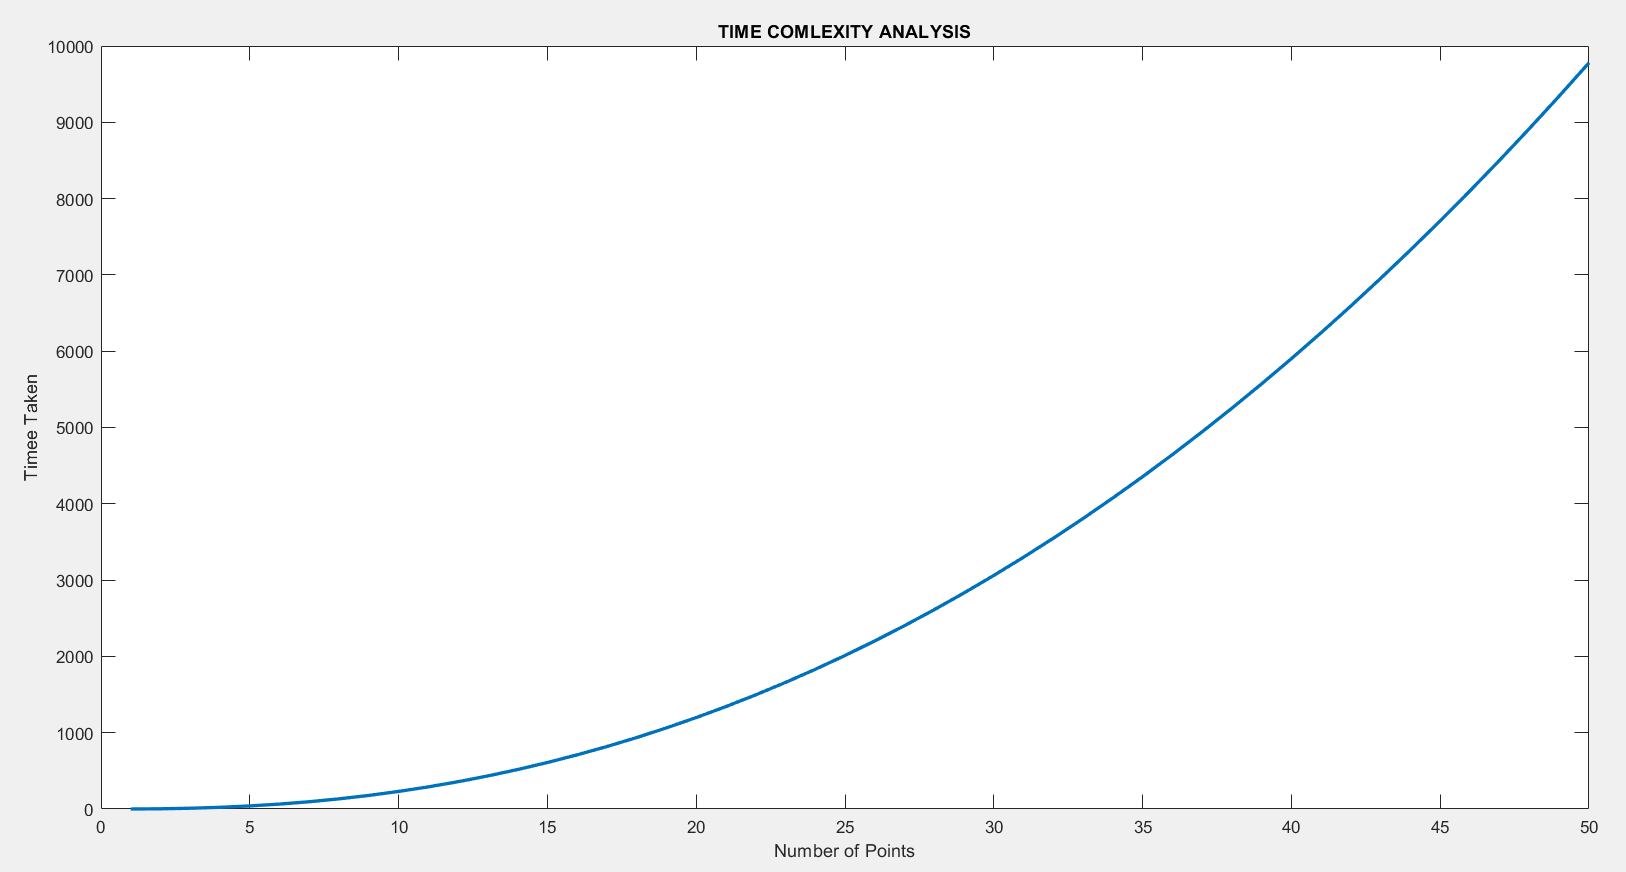
\includegraphics[width=\columnwidth, height=6cm]{Time Complexity.png}\begin{center}\textbf{Figure 3:} Time Complexity Graph\end{center}By the experimental analysis, we found that in  case of optimized approach, on increasing the no. of points in the set (increasing the size of set) the graph is strictly increasing with a bend (or concavity) towards horizontal axis. Thus the overall time increases with an increase in no. of points.

\paragraph{Space Analysis:}Following is the graph representing the space complexity of the algorithm.\\\\\\
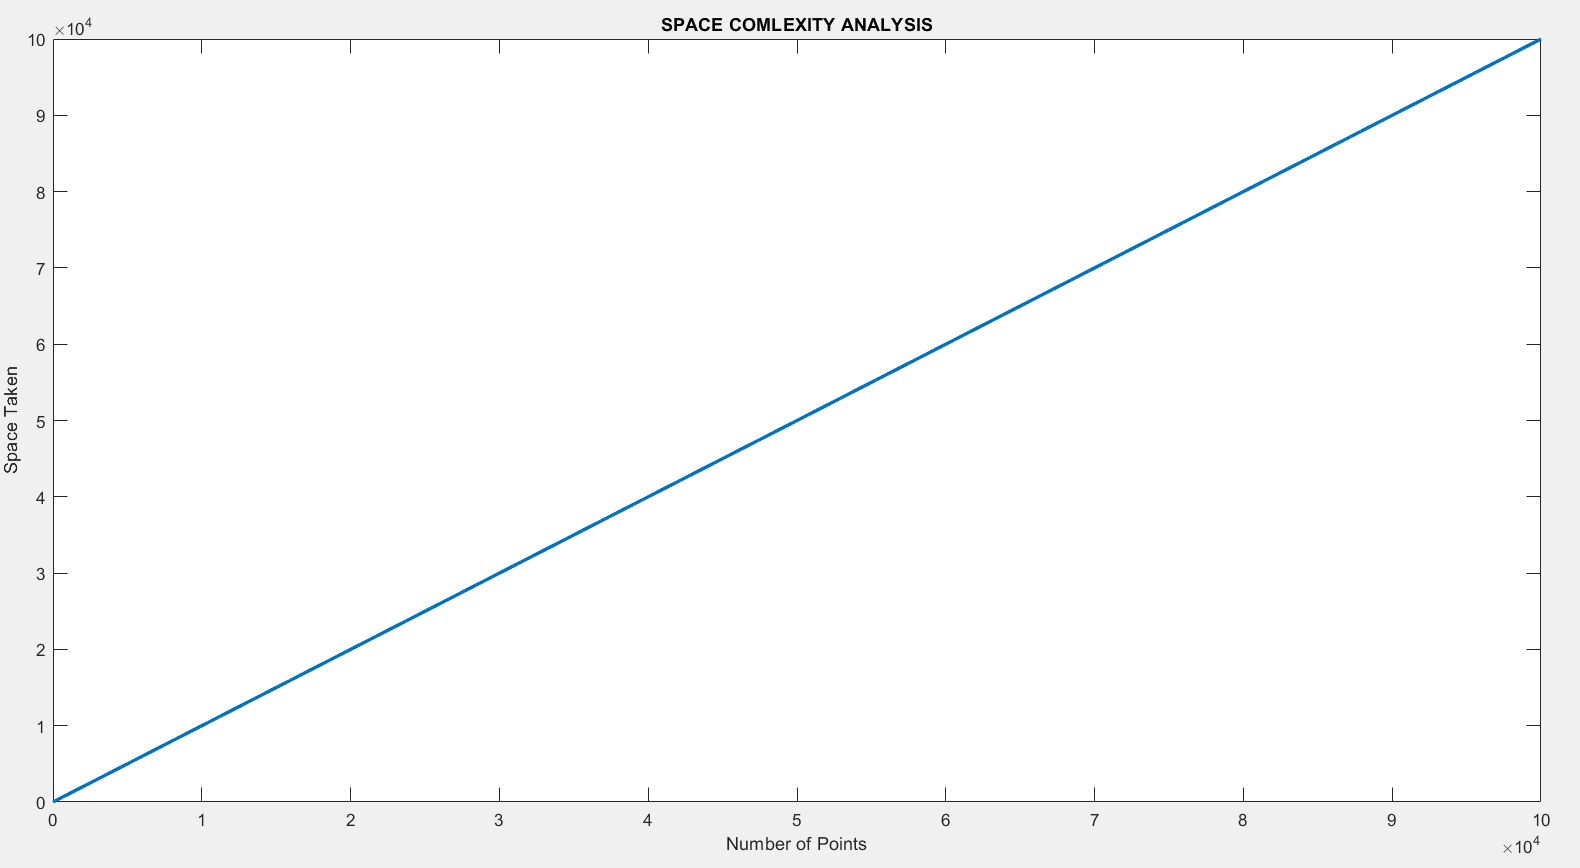
\includegraphics[width=\columnwidth, height=6cm]{Space Complexity.png}\begin{center}\textbf{Figure 4:} Space Complexity Graph\end{center}By the experimental analysis, we found that in case of optimized approach, on increasing the no. of points in the set (increasing the size of set) the graph is strictly increasing Thus the overall space increases with an increase in no. of points.\\\\

\paragraph{CONCLUSION:} \\


So, with the above mentioned algorithms and their profiling, we come to the conclusion that this classical problem of finding the  area of n-sided polygon is achieving its best time complexity of O(nlogn) and space complexity of O(n).\\\\ Hence this is one of the most effiicient way to find area of polygon.

\section*{REFERENCES}


\begin{enumerate}
    
\item  \href{https://www.geeksforgeeks.org/divide-and-conquer-algorithm-introduction/}{Divide and Conquer}
\item  \href{https://en.wikipedia.org/wiki/Shoelace_formula}{Shoelace_formula}\\

\end{enumerate}\\

\end{multicols*}

\clearpage

\end{document}
